%%%%%%%%%%%%%%%%%%%%%%%%%%%%%%%%%%%%%%%%%
% Structured General Purpose Assignment
% LaTeX Template
%
% This template has been downloaded from:
% http://www.latextemplates.com
%
% Original author:
% Ted Pavlic (http://www.tedpavlic.com)
%
% Note:
% The \lipsum[#] commands throughout this template generate dummy text
% to fill the template out. These commands should all be removed when 
% writing assignment content.
%
%%%%%%%%%%%%%%%%%%%%%%%%%%%%%%%%%%%%%%%%%

%----------------------------------------------------------------------------------------
%	PACKAGES AND OTHER DOCUMENT CONFIGURATIONS
%----------------------------------------------------------------------------------------

\documentclass{article}

\usepackage{fancyhdr} % Required for custom headers
\usepackage{lastpage} % Required to determine the last page for the footer
\usepackage{extramarks} % Required for headers and footers
\usepackage{graphicx} % Required to insert images
\usepackage{lipsum} % Used for inserting dummy 'Lorem ipsum' text into the template
\usepackage{enumerate}
\usepackage{booktabs}
\usepackage{amsmath}
\usepackage{subcaption}
\usepackage{tikz}
\usetikzlibrary{matrix}

% Margins
\topmargin=-0.45in
\evensidemargin=0in
\oddsidemargin=0in
\textwidth=6.5in
\textheight=9.0in
\headsep=0.25in 

\linespread{1.5} % Line spacing

% Set up the header and footer
\pagestyle{fancy}
\lhead{\hmwkAuthorName} % Top left header
\chead{\hmwkClass\ (\hmwkTitle)} % Top center header
%%\rhead{\firstxmark} 
\rhead{} % Top right header
\lfoot{\lastxmark} % Bottom left footer
\cfoot{} % Bottom center footer
\rfoot{Page\ \thepage\ of\ \pageref{LastPage}} % Bottom right footer
\renewcommand\headrulewidth{0.4pt} % Size of the header rule
\renewcommand\footrulewidth{0.4pt} % Size of the footer rule

\setlength\parindent{0pt} % Removes all indentation from paragraphs

%----------------------------------------------------------------------------------------
%	DOCUMENT STRUCTURE COMMANDS
%	Skip this unless you know what you're doing
%----------------------------------------------------------------------------------------

% Header and footer for when a page split occurs within a problem environment
\newcommand{\enterProblemHeader}[1]{
\nobreak\extramarks{#1}{#1 continued on next page\ldots}\nobreak
\nobreak\extramarks{#1 (continued)}{#1 continued on next page\ldots}\nobreak
}

% Header and footer for when a page split occurs between problem environments
\newcommand{\exitProblemHeader}[1]{
\nobreak\extramarks{#1 (continued)}{#1 continued on next page\ldots}\nobreak
\nobreak\extramarks{#1}{}\nobreak
}

\setcounter{secnumdepth}{0} % Removes default section numbers
\newcounter{homeworkProblemCounter} % Creates a counter to keep track of the number of problems

\newcommand{\homeworkProblemName}{}
\newenvironment{homeworkProblem}[1][Problem \arabic{homeworkProblemCounter}]{ % Makes a new environment called homeworkProblem which takes 1 argument (custom name) but the default is "Problem #"
\stepcounter{homeworkProblemCounter} % Increase counter for number of problems
\renewcommand{\homeworkProblemName}{#1} % Assign \homeworkProblemName the name of the problem
\section{\homeworkProblemName} % Make a section in the document with the custom problem count
\enterProblemHeader{\homeworkProblemName} % Header and footer within the environment
}{
\exitProblemHeader{\homeworkProblemName} % Header and footer after the environment
}

\newcommand{\problemAnswer}[1]{ % Defines the problem answer command with the content as the only argument
\noindent\framebox[\columnwidth][c]{\begin{minipage}{0.98\columnwidth}#1\end{minipage}} % Makes the box around the problem answer and puts the content inside
}

\newcommand{\homeworkSectionName}{}
\newenvironment{homeworkSection}[1]{ % New environment for sections within homework problems, takes 1 argument - the name of the section
\renewcommand{\homeworkSectionName}{#1} % Assign \homeworkSectionName to the name of the section from the environment argument
\subsection{\homeworkSectionName} % Make a subsection with the custom name of the subsection
\enterProblemHeader{\homeworkProblemName\ [\homeworkSectionName]} % Header and footer within the environment
}{
\enterProblemHeader{\homeworkProblemName} % Header and footer after the environment
}

%----------------------------------------------------------------------------------------
%	BINOMIAL TREE
%----------------------------------------------------------------------------------------

% Set the overall layout of the tree
\tikzstyle{level 1}=[level distance=4cm, sibling distance=3.5cm,->]
\tikzstyle{level 2}=[level distance=4cm, sibling distance=2cm,->]
 
% Define styles for bags and leafs
\tikzstyle{bag} = [text width=2em, text centered]
\tikzstyle{end} = []
 
% The sloped option gives rotated edge labels. Personally
% I find sloped labels a bit difficult to read. Remove the sloped options
% to get horizontal labels.    
%----------------------------------------------------------------------------------------
%	NAME AND CLASS SECTION
%----------------------------------------------------------------------------------------

\newcommand{\hmwkTitle}{Homework\ \#4} % Assignment title
\newcommand{\hmwkDueDate}{Tuesday,\ February\ 20,\ 2018} % Due date
\newcommand{\hmwkClass}{FIN\ 513} % Course/class
\newcommand{\hmwkClassTime}{9:30am} % Class/lecture time
\newcommand{\hmwkAuthorName}{Wanbae Park} % Your name

%----------------------------------------------------------------------------------------
%	TITLE PAGE
%----------------------------------------------------------------------------------------

\title{
\vspace{2in}
\textmd{\textbf{\hmwkClass:\ \hmwkTitle}}\\
\normalsize\vspace{0.1in}\small{Due\ on\ \hmwkDueDate}\\
\vspace{3in}
}

\author{\textbf{\hmwkAuthorName}}
\date{} % Insert date here if you want it to appear below your name

%----------------------------------------------------------------------------------------

\begin{document}

\maketitle

%----------------------------------------------------------------------------------------
%	TABLE OF CONTENTS
%----------------------------------------------------------------------------------------

%\setcounter{tocdepth}{1} % Uncomment this line if you don't want subsections listed in the ToC

%%\newpage
%%\tableofcontents
\newpage

%----------------------------------------------------------------------------------------
%	PROBLEM 1
%----------------------------------------------------------------------------------------

% To have just one problem per page, simply put a \clearpage after each problem

\begin{homeworkProblem}
	\begin{enumerate}[(a)]
	\item
	By using the formula $u = e^{\sigma \sqrt{\Delta t}}$ and $d = 1/u$, the binomial tree is constructed and by using backward induction, price of call option was calculated as 0.0561506, price of put option was calculated as 0.0659037. Since a straddle is a portfolio of a call and put for long position both, price of straddle is calculated as 0.0561506 + 0.0659037 = 0.122054.
	\item	
	Using the same tree constructed in (a), straddle price is calculated by same method with each maturity, and plotted as Figure \ref{fig:prob1 - straddle price}. It seems that $\frac{\partial \Pi}{\partial t}$ has negative value since price of straddle is decreasing.
	%% Straddle price plot
	\begin{figure}[h]
	\centering
		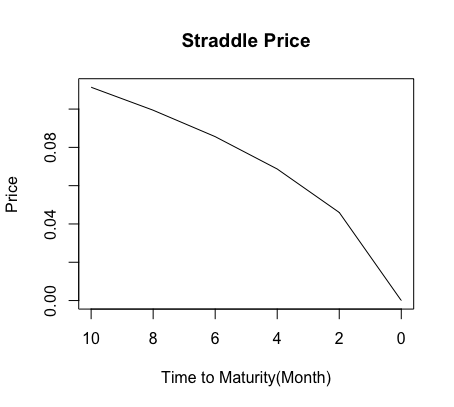
\includegraphics[scale = 0.6]{straddle_price.png}
		\caption{Straddle price}
	\label{fig:prob1 - straddle price}
	\end{figure}
	%%
	\item
	Even though the price of straddle is decreasing on the plot, it does not mean buying a straddle has a negative expected return. It is because the values of straddle corresponding maturity were calculated assuming \underline{others are equal}. Since straddle has positive payoff unless underlying price at maturity is exactly same as price at initial date, it is likely to make a profit if variation of stock price is high enough. However, since Figure \ref{fig:prob1 - straddle price} ignores variation of underlying prices, it seems that holding a straddle makes negative return even if it is not true.
	\end{enumerate}
\end{homeworkProblem}

%----------------------------------------------------------------------------------------
%	PROBLEM 2
%----------------------------------------------------------------------------------------
\begin{homeworkProblem}
\end{homeworkProblem}

%----------------------------------------------------------------------------------------
%	PROBLEM 3
%----------------------------------------------------------------------------------------
\begin{homeworkProblem}
	\textbf{False.} It is not necessary to assume the options are not marked to market. The only assumption to derive options prices under binomial model is that underlying asset and riskless bond are tradable(both long and short) at each steps. Regardless of marking-to-market, it is possible to price option only if we can replicate payoff of options by trading underlying asset and riskless bond at each node.
\end{homeworkProblem}

%----------------------------------------------------------------------------------------
%	PROBLEM 4
%----------------------------------------------------------------------------------------
\begin{homeworkProblem}
	\begin{enumerate}[a.]
	%% Sub-Problem a.
	\item
	Let $\bar{r}^d$ and $\bar{r}^f$ denote gross return of domestic riskless bond and foreign riskless bond, respectively. Then the risk-neutral probability $\bar{q}$ is calculated as $\bar{q} = \frac{\bar{r}^d / \bar{r}^f - d}{u - d}$.
	\begin{enumerate}[i.]
		\item
		\textit{Assume $\bar{q} > 1$.} Since $u - d > 0$, $\bar{q} = \frac{\bar{r}^d / \bar{r}^f - d}{u - d} > 1$ is equivalent to $\frac{\bar{r}^d}{\bar{r}^f} - d > u - d \Rightarrow \frac{\bar{r}^d}{\bar{r}^f} > u > d$. Using this inequality, it is possible to make an arbitrage profit using the following strategies.
		\begin{enumerate}[(1)]
			\item Borrow an foreign currency and exchange to domestic currency.
			\item Invest domestic currency from exchange of foreign currency to riskless bond.
		\end{enumerate}
		After one period, assume that the exchange rate becomes higher to $S_t \times u$. Then the investor have to pay $S_t u \bar{r}^f$ to the lender, and gets $S_t \bar{r}^d$ from the investment of domestic riskless bond. Therefore, the final payoff of the strategy is equal to $S_t \bar{r}^d - S_t u \bar{r}^f = S_t(\bar{r}^d / \bar{r}^f - u)$. Because we assumed that $\bar{r}^d / \bar{r}^f - u > 0$, and there is no initial cost to make the portfolio, the investor can make an arbitrage profit. Case in which exchange rate becomes $S_t \times d$ is analogous.
		\item
		\textit{Assume $\bar{q} < 0$.}
		$\bar{q} = \frac{\bar{r}^d / \bar{r}^f - d}{u - d} < 0$ is equivalent to $\frac{\bar{r}^d}{\bar{r}^f} - d < 0 \Rightarrow \frac{\bar{r}^d}{\bar{r}^f}  < d < u$. In this case, it is also possible to make an arbitrage profit using the following strategies.
		\begin{enumerate}[(1)]
			\item Borrow $S_t$ amount of domestic currency and exchange into a foreign currency.
			\item Invest a foreign currency to riskless bond.
		\end{enumerate}
		Then after one period, assuming the exchange rate becomes to $S_t \times d$, the investor will get $S_t d \bar{r}^f$ and have an obligation to pay $S_t \bar{r}^d$. Therefore, the final payoff the strategy is equal to $S_t d \bar{r}^f - S_t \bar{r}^d = S_t(d - \bar{r}^d / \bar{r}^f)$, which is positive. Therefore, the investor can make an arbitrage profit since there is no initial amount of investment. Case in which exchange rate becomes $S_t \times u$ is analogous.
	\end{enumerate}
	%% Sub-Problem b.	
	\item
	First, let us assume that exchange rate $y$ becomes $y \times u$ or $y \times d$ after one month. Assuming the expect return of investing in Afghani is zero, in order to match the expected return, the following equation should hold.
	\begin{equation*}
		y = 0.5 \times yu + 0.5 \times yd
	\end{equation*}
	Cancelling $y$ out on both sides and rearranging the terms, equation $d = 2 - u$ is obtained. Using the result, in order to match standard deviation, we can construct the following equation.
	\begin{equation*}
	\begin{aligned}
		&0.5 \times u^2 + 0.5 \times d^2 = 0.5 \times u^2 + 0.5 \times (2 - u)^2 = \frac{0.1}{12} \approx 0.008	\\
		&\Rightarrow u^2 - 2u + 2 - 0.008 = 0	\\
		&\Rightarrow u = \frac{2 \pm \sqrt{4 - (1.992)^2}}{2} = 1.089~\text{or}~0.910
	\end{aligned}
	\end{equation*}
	Since $u > d$, $u = 1.089$ and $d = 2 - u = 0.910$. By using the given interest rate to calculate risk-neutral probability $\bar{q}$, it is calculated as $\bar{q} = \frac{1.02 / 1.08 - 0.910}{1.089 - 0.910} = 0.1924$, which is between 0 and 1, satisfies the condition derived in (a). Therefore, if the value of $u$ and $d$ calculated above are used for constructing tree, it is possible to match the moments of exchange rate.
	\end{enumerate}
\end{homeworkProblem}

%----------------------------------------------------------------------------------------
%	PROBLEM 5
%----------------------------------------------------------------------------------------
\begin{homeworkProblem}
\end{homeworkProblem}
\begin{enumerate}[a.]
	\item
	Using the formula $u = e^{\sigma \Delta t}$, $d = 1/ u$, a tree is constructed(Figure \ref{tree:prob5-stockprice}). However, since volatility changes at each nodes, $u$ and $d$ changes(as shown on Figure \ref{tree:prob5-vol and u}), it does no longer recombines, consequently.
%----------------------------------------------------------------------------------------
	%% STOCK PRICE TREE
	\begin{figure}[h]
	\centering
	\begin{tikzpicture}[grow=right, sloped]
	\node[bag] {20}
     	child {
        	 node[bag] {12.13}        
        	     child {
        	         node[end, label=right:
        	             {6.38}] {}
        	         edge from parent
        	         node[above] {}
        	         node[below]  {}
        	     }
        	     child {
        	         node[end, label=right:
        	             {23.05}] {}
        	         edge from parent
        	         node[above] {}
        	         node[below] {}
        	     }
        	     edge from parent 
        	     node[above] {}
        	     node[below]  {}
     	}
     	child {
        	 node[bag] {32.97}        
        	 child {
        	         node[end, label=right:
        	             {22.34}] {}
        	         edge from parent
        	         node[above] {}
        	         node[below]  {}
        	     }
        	     child {
        	         node[end, label=right:
        	             {48.67}] {}
        	         edge from parent
        	         node[above] {}
        	         node[below]  {}
        	     }
        	 edge from parent         
        	     node[above] {}
        	     node[below]  {}
     	};
	\end{tikzpicture}
	\caption{Stock price tree}
	\label{tree:prob5-stockprice}
	\end{figure}
%----------------------------------------------------------------------------------------
	%% VOLATILITY AND U TREE
	\begin{figure}[h]
	\centering
	\begin{subfigure}[b]{0.4\linewidth}
		\begin{tikzpicture}[grow=right, sloped]
		\node[bag] {0.5}
     		child {
        	 	node[bag] {0.6420}       
        	 	    edge from parent 
    	    	     node[above] {}
        		     node[below]  {}
    		 }
		     child {
    	    	 node[bag] {0.3894}        
    	    	 edge from parent         
      	  	     node[above] {}
     	   	     node[below]  {}
    	 	};
		\end{tikzpicture}%
		\caption{Volatility Tree}
		\label{tree:prob5-volatility}
	\end{subfigure}
	\begin{subfigure}[b]{0.4\linewidth}
	\begin{tikzpicture}[grow=right, sloped]
	\node[bag] {1.649}
	     child {
       	  node[bag] {1.900}       
        	     edge from parent 
        	     node[above] {}
        	     node[below]  {}
     	}
	     child {
        	 node[bag] {1.476}        
        	 edge from parent         
        	     node[above] {}
        	     node[below]  {}
     	};
	\end{tikzpicture}
	\caption{$u$ Tree}
	\end{subfigure}
	\label{tree:prob5-u}
	\caption{Volatility and $u$}
	\label{tree:prob5-vol and u}
	\end{figure}
%----------------------------------------------------------------------------------------
	Since there are 4 states at period 2, there are four possible returns and corresponding probabilities. Tables \ref{tab:returns and probs} represents returns and probabilities at each states.
%----------------------------------------------------------------------------------------
	%% RETURNS AND PROBS
	\begin{table}[]
	\centering
	\label{my-label}
	\begin{tabular}{@{}ccc@{}}
	\toprule
	\textit{Stock Price} & \textit{Return($r$)} & \textit{Probability($p$)} \\ \midrule
	48.67                & 1.434           & 0.3025               \\
	22.34                & 0.117           & 0.2475               \\
	23.05                & 0.153           & 0.2475               \\
	6.38                 & -0.681          & 0.2025               \\ \bottomrule
	\end{tabular}
	\caption{Returns and probabilities at each state}
	\label{tab:returns and probs}
	\end{table}
	From the table, since returns and probabilities at each state are given, it is possible to calculate expected return and variance. Expected return is calculated as $\mathrm{E}(r) = \sum_{i = 1}^4 r_i p_i = 1.434 \times 0.3025 + 0.117 \times 0.2475 + 0.153 \times 0.2475 -0.681 \times 0.2025 = 36.25\%$, Variance is calculated as $\mathrm{Var}(r) = \sum_{i = 1}^4 (r_i - \mathrm{E}(r))^2 = 59.33\%$. Therefore, standard deviation is equal to $\sqrt{59.33}\% = 77.03\%$, and annualized variance and volatility is equal to $29.67\%$ and $54.47\%$, respectively.
	%%
	\item
	Since the volatility changes at each node, risk neutral probability $q$ would change at each nodes, and it affects value of the option. Figure \ref{tree:prob5-risk-neutral probs} represents risk-neutral probabilities at each node.
	%% RISK-NEUTRAL PROB TREE
	\begin{figure}[h]
	\centering
		\begin{tikzpicture}[grow=right, sloped]
		\node[bag] {0.3872}
     		child {
        	 	node[bag] {0.3521}       
        	 	    edge from parent 
    	    	     node[above] {}
        		     node[below]  {}
    		 }
		     child {
    	    	 node[bag] {0.4164}        
    	    	 edge from parent         
      	  	     node[above] {}
     	   	     node[below]  {}
    	 	};
		\end{tikzpicture}
		\caption{Risk-neutral probabilities}
		\label{tree:prob5-risk-neutral probs}
	\end{figure}
	Using risk-neutral probabilities at each node and backward induction formula $c = \frac{1}{1 + r_f}(q \times c_u + (1 - q) \times c_d)$, it is possible to value the call option. ($c$ = value of option at previous node, $c_u$, and $c_d$ represents value of option at up-state and down-state. $r_f$ is risk-free rate.) Figure \ref{tree:prob5-optionprice} shows valuation process using the backward induction procedure.
%----------------------------------------------------------------------------------------
	%% OPTION PRICE TREE
	\begin{figure}[h]
	\centering
	\begin{tikzpicture}[grow=right, sloped]
	\node[bag] {5.696}
     	child {
        	 node[bag] {1.064}        
        	     child {
        	         node[end, label=right:
        	             {0}] {}
        	         edge from parent
        	         node[above] {}
        	         node[below]  {}
        	     }
        	     child {
        	         node[end, label=right:
        	             {3.052}] {}
        	         edge from parent
        	         node[above] {}
        	         node[below] {}
        	     }
        	     edge from parent 
        	     node[above] {}
        	     node[below]  {}
     	}
     	child {
        	 node[bag] {13.174}        
        	 child {
        	         node[end, label=right:
        	             {2.339}] {}
        	         edge from parent
        	         node[above] {}
        	         node[below]  {}
        	     }
        	     child {
        	         node[end, label=right:
        	             {28.673}] {}
        	         edge from parent
        	         node[above] {}
        	         node[below]  {}
        	     }
        	 edge from parent         
        	     node[above] {}
        	     node[below]  {}
     	};
	\end{tikzpicture}
	\caption{Option price tree}
	\label{tree:prob5-optionprice}
	\end{figure}
	From the tree, the option value is calculated as 5.696 when volatility is not constant.
%----------------------------------------------------------------------------------------
	%% STOCK PRICE TREE: CONST VOL
	\begin{figure}[h]
	\centering
	\begin{tikzpicture}[>=stealth,sloped]
		\matrix (tree) [%
		matrix of nodes,
		minimum size=1cm,
		column sep=3.5cm,
		row sep=1cm,
    	]
    	{
        				  &   & 59.45 \\
	       	  	 & 34.48 &   \\
	      \$20.00 & 	 	 & 20.00 \\
        		 	 & 11.60 &   \\
		       		   &   & 6.73 \\
    };
    \draw[->] (tree-3-1) -- (tree-2-2) node [midway,above] {};
    \draw[->] (tree-3-1) -- (tree-4-2) node [midway,below] {};
    \draw[->] (tree-2-2) -- (tree-1-3) node [midway,above] {};
    \draw[->] (tree-2-2) -- (tree-3-3) node [midway,below] {};
    \draw[->] (tree-4-2) -- (tree-3-3) node [midway,above] {};
    \draw[->] (tree-4-2) -- (tree-5-3) node [midway,below] {};
  	\end{tikzpicture}
  	\caption{Stock price tree: constant volatility}
	\label{tree:prob5-stock price tree: const volatility}
  	\end{figure}
%----------------------------------------------------------------------------------------
	%% OPTION PRICE TREE: CONST VOL
	\begin{figure}[h]
	\centering
	\begin{tikzpicture}[>=stealth,sloped]
		\matrix (tree) [%
		matrix of nodes,
		minimum size=1cm,
		column sep=3.5cm,
		row sep=1cm,
    	]
    	{
        				  &   & 39.45 \\
	       	  	 & 14.680 &   \\
	      \$5.463 & 	 	 & 0 \\
        		 	 & 0 &   \\
		       		   &   & 0 \\
    };
    \draw[->] (tree-3-1) -- (tree-2-2) node [midway,above] {};
    \draw[->] (tree-3-1) -- (tree-4-2) node [midway,below] {};
    \draw[->] (tree-2-2) -- (tree-1-3) node [midway,above] {};
    \draw[->] (tree-2-2) -- (tree-3-3) node [midway,below] {};
    \draw[->] (tree-4-2) -- (tree-3-3) node [midway,above] {};
    \draw[->] (tree-4-2) -- (tree-5-3) node [midway,below] {};
  	\end{tikzpicture}
  	\caption{Option price tree: constant volatility}
	\label{tree:prob5-option price tree: const volatility}
  	\end{figure}
\end{enumerate}
\end{document}
